\section{Emissioni}

Qui di seguito vengono riportate le emissioni di CO2 per ogni esperimento effettuato.

\begin{table}[H]
    \centering
    \footnotesize
    \setlength\tabcolsep{0pt}
    \begin{tabularx}{\textwidth}{|X|X|}
        \hline
        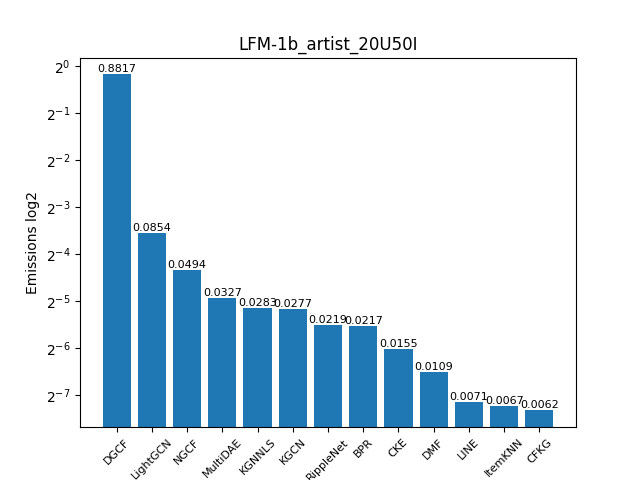
\includegraphics[width=\linewidth, trim=0 0 0 0]{images/emissions_LFM-1b_artist_20U50I.png} &
        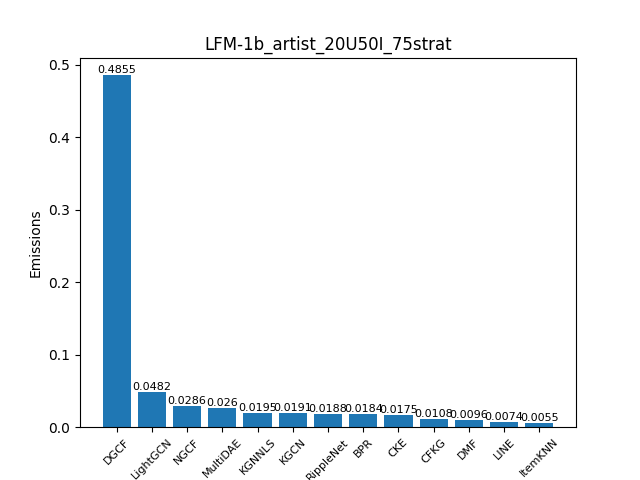
\includegraphics[width=\linewidth, trim=0 0 0 0]{images/emissions_LFM-1b_artist_20U50I_75strat.png} \\
        \hline
        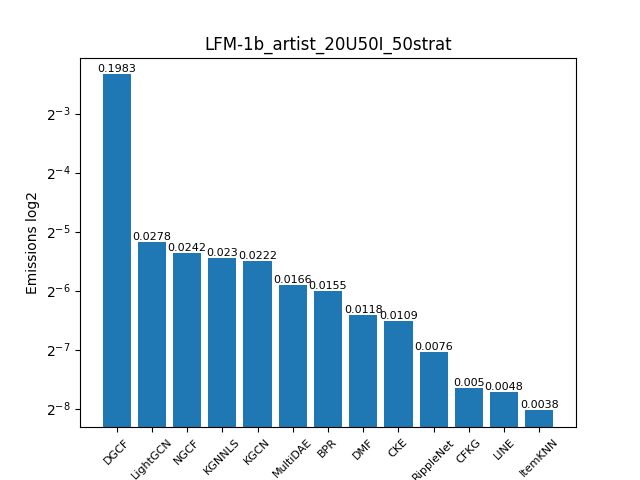
\includegraphics[width=\linewidth, trim=0 0 0 0]{images/emissions_LFM-1b_artist_20U50I_50strat.png} &
        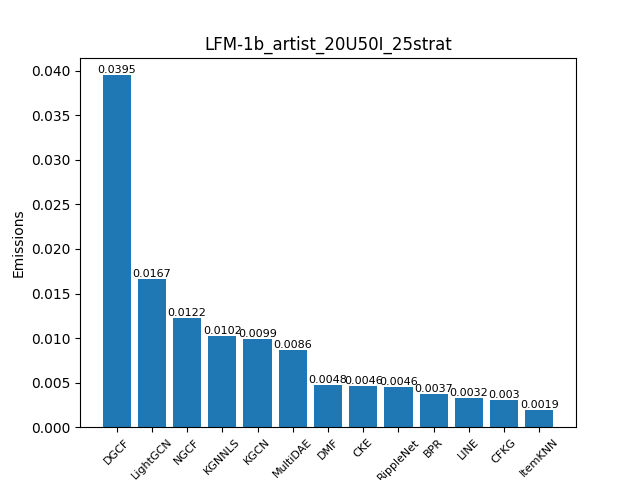
\includegraphics[width=\linewidth, trim=0 0 0 0]{images/emissions_LFM-1b_artist_20U50I_25strat.png} \\
        \hline
    \end{tabularx}
    \caption{Emissioni di CO2 per i vari dataset}
    \label{tab:emissions_info}
\end{table}

\noindent Si può subito notare come DGCF è il modello che emette più CO2 in assoluto.
In particolare con il dataset al 100\% e al 75\% DGCF emette circa 10 volte di più rispetto a LightGCN (il secondo per emissioni)
mentre con il dataset al 50\% emette circa 7 volte di più e con il dataset al 25\% emette circa 2 volte di più (sempre rispetto a LightGCN).
Questo non dovrebbe sorprendere in quanto DGCF utilizza un knowledge graph e lavora su di essi creando rappresentazioni disgiunte.
LightGCN e NCFG sono rispettivamente il secondo e il terzo modello che emettono più CO2.
Questi due modelli sono invece di tipo general, ma nonostante ciò emettono di più rispetto ad altri di tipo knowledge-aware, come per esempio il KGCN.
In generale possiamo vedere che ItemKNN,LINE e CFKG sono i modelli che emettono meno.
Per LINE e ItemKNN questo era abbastanza prevedibile in quanto modelli di tipo General. Interessante invece notare come CFKG, di tipo knowledge-aware, emetta meno di altri modelli di tipo General





